\documentclass[12pt]{article}
\usepackage{amsmath}
\usepackage{csvsimple}
\usepackage{graphicx}
\graphicspath{ {./../images/} }
\usepackage{hyperref}
\usepackage[latin1]{inputenc}
\usepackage{listings}

\DeclareMathOperator{\Tr}{Tr}

\lstset{
  columns=fullflexible,
  breaklines=true,
}

\title{Local Assortativity on Networks with Unbalanced Classes}
\author{Rebecca Cohen}

\begin{document}
\maketitle
\section{Abstract}
\section{Introduction}

\section{Multiscale Mixing In Unbalanced Classes}
Include simulations and real data

\section{Modularity in Unbalanced Classes}
Include experiments with $\gamma$
Reflections on modularity and edge counts vs. pairing probability

\section{Adjustments}
Weighting $a_r$.  Theory and results.  Drop this?

\section{Blockwise Expectation of Multiscale Mixing Scores Under DC-SBM}
The multiscale mixing score $r(\ell)$ is defined
\begin{equation}
  r(\ell) = \frac{1}{Q_{max}} \sum_g (e_{gg}(\ell) - a_g^2)
\end{equation}

where 
\begin{equation}
  e_{gg}(\ell) = \sum_i \sum_j w_{\text{multi}}(i; \ell) \frac{A_{ij}}{k_i} \delta(z_i, z_j) 
\end{equation}

and $k_i$ is the degree of the ith node, while $w_{\text{multi}}(i; \ell)$ is the $i$th element of the totalRank vector centered at node $\ell$.  With two key assumptions, we can calculate the expectation of $r(\ell)$ under a degree-corrected stochastic block model (DC-SBM).  While neither is assumption is true in general, numerical simulations support the predictions resulting from this calculation:

\begin{enumerate}
  \item The degree of every node is equal to its expected degree ($k_i = \theta_i$)
  \item The network is fully connected
\end{enumerate}

Assumption 1 allows us to treat node degrees and edge counts as constants.  Without this assumption, both $e_gg(\ell)$ and $a_g$ are the ratios of two Poisson random variables, and it is theoretically possible for the denominator to equal 0, rendering the expectations of these measures undefined.  However, on networks large enough to be interesting, the edge count is extremely unlikely to be zero, and tends to be close to its expectation under the DC-SBM.  More work is needed to develop probabilistic bounds on the error, but numerical simulations support the utility of this naive appoximation (see figure BLAH).    

Assumption 2 will become necessary when we compute transition probabilities for the blockwise personalized pageRank. 

ALTERNATE FRAMING: random rewiring of an empirical network.

TODO: Define the DC-SBM parameters

Under this simplified regime, since every node has its expected degree,
\begin{equation}
  a_g = \sum_i \sum_j A_{ij} \delta(z_i, g) = \sum_h \mathcal{M}_{gh}
\end{equation}

Noteably, $a_g$ is a constant here so 
\begin{equation}
  \langle r(\ell) \rangle = \frac{\langle e_{gg}(\ell) \rangle - \sum_g \big( \mathcal{M}_{gh} \big)}{1 - \sum_g \big( \mathcal{M}_{gh} \big)}
\end{equation}

To compute the expectation of $e_{gg}(\ell)$, we build on recent work by Chen et al \cite{chen:2020} showing that
\begin{equation}
  \langle w_\alpha (i ; \ell) \rangle = \theta_i w_\alpha(g)
\end{equation}
where $w_\alpha(i;\ell)$ is the personalized pageRank of node $i$ with respect to node $\ell$ given a fixed $\alpha$, and $w_\alpha$ is the blockwise personalized pageRank.

TODO: blockwise PPR! 

so for a given $\alpha$, $\theta_i$ and $k_i$ cancel, and
\begin{equation}
  \begin{aligned}
    \langle e_{\alpha, gg}(\ell) \rangle &= \sum_i \sum_j w_\alpha(z_i; \ell) A_{ij} \delta{z_i, z_j} \\
    &= w_\alpha(g; \ell) \sum_i \sum_j A_{ij} \delta{z_i, z_j} \\
    &= w_\alpha(g; \ell) \mathcal{M}_{gg}
  \end{aligned}
\end{equation}

Since totalRank is the integral of personalized pageRank over $\alpha \in [0,1]$ \cite{boldi:2005} \cite{Peel:2018}, we use the linearity of integration and expectation to conclude
\begin{equation}
  \langle e_{gg}(\ell) \rangle = \mathcal{M}_{gg} w(g; \ell) 
\end{equation}

where $w(g; \ell) = \int_0^1 w_\alpha(g; \ell)$.  This can be easily be approximated numerically.  Since $w_\alpha (g;\ell)$ can be computed in just $O(C^2)$, this integral can easily be approximated numerically from the results for many choices of $\alpha$.

Substituting the expection of $\langle e_{gg}(\ell)\rangle$ back into equation NUMBER, we find

\begin{equation}
  \langle r(\ell) \rangle = \frac{\mathcal{M}_{gg} w(g; \ell) - \sum_g \big( \mathcal{M}_{gh} \big)}{1 - \sum_g \big( \mathcal{M}_{gh} \big)}
\end{equation}

Equation NUMBER depends only on the mixing matrix and blockwise PPR vector.  This means that $\langle r(\ell) \rangle$ will be the same for every element of each block, regardless of its degree.  It also means that we can compute $\langle r(\ell) \rangle$ directly from the mixing matrix.

\section{Numerical Experiments}
The calculation above relied on two highly unrealistic assumptions about the DC-SBM.  However, formula NUMBER 

\begin{figure}[h!]
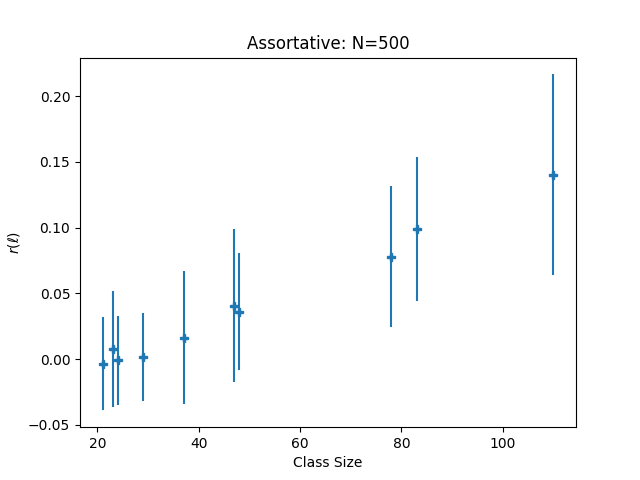
\includegraphics[width=0.5\textwidth]{assortative_N_500.png}
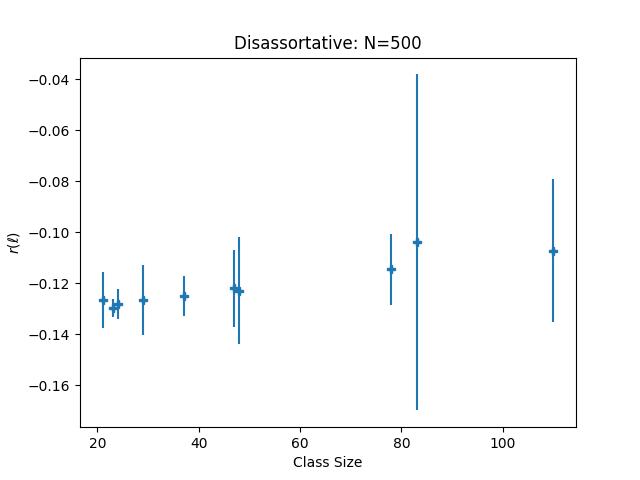
\includegraphics[width=0.5\textwidth]{disassortative_N_500.png}
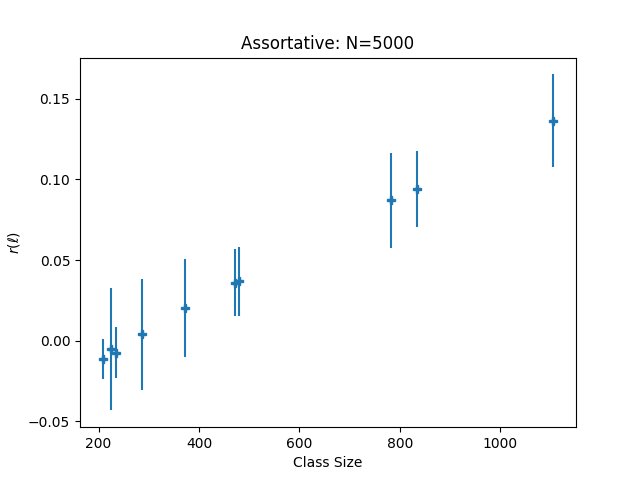
\includegraphics[width=0.5\textwidth]{assortative_N_5000.png}
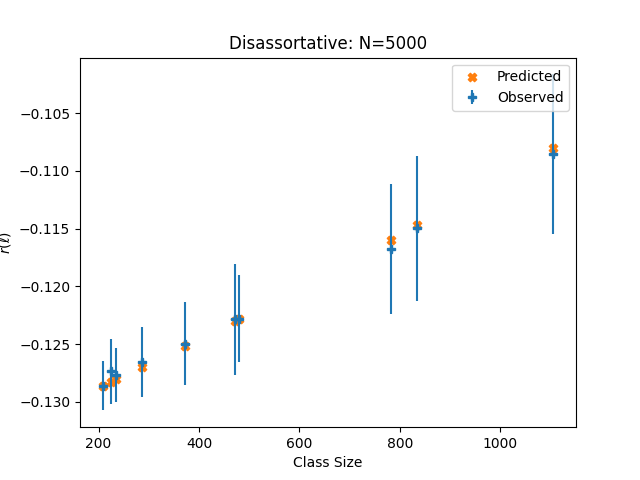
\includegraphics[width=0.5\textwidth]{disassortative_N_5000.png}
\caption{Distribution of $r(\ell)$ on DC-SBM random networks with uneven class sizes and heavy-tailed degree distribution.  Networks are constructed to have similar proportions within each class and similar in- and out-group pairing probabilities}
\end{figure}

\begin{figure}[h!]
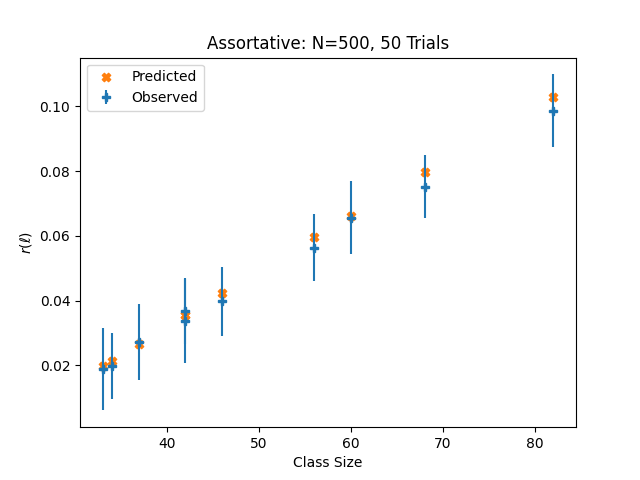
\includegraphics[width=0.5\textwidth]{assortative_N_500_trials_50.png}
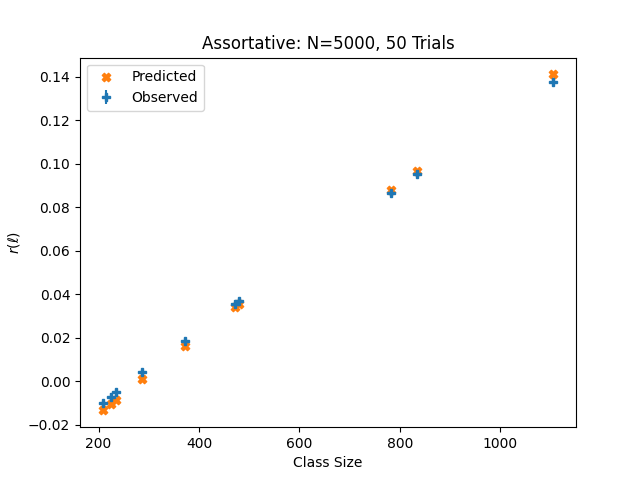
\includegraphics[width=0.5\textwidth]{assortative_N_5000_trials_50.png}
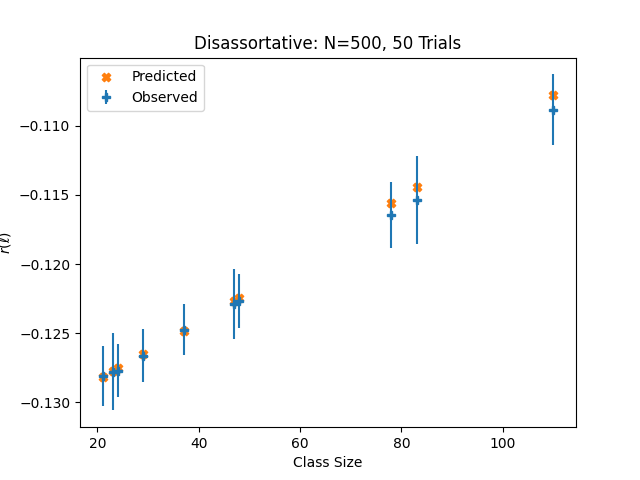
\includegraphics[width=0.5\textwidth]{disassortative_N_500_trials_50.png}
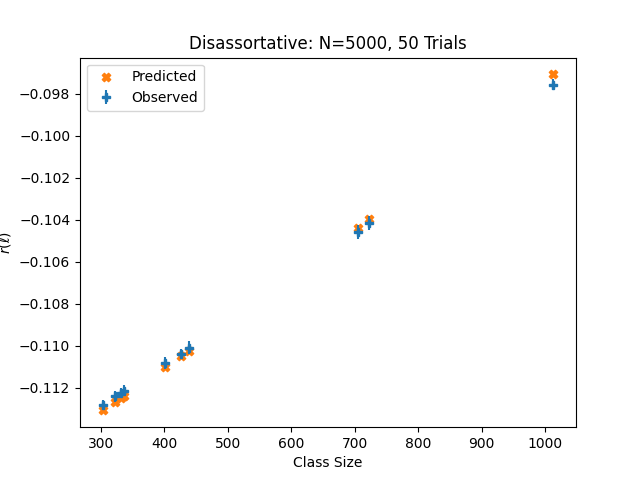
\includegraphics[width=0.5\textwidth]{disassortative_N_5000_trials_50.png}
\caption{Classwise mean $r(\ell)$ across 50 trials on DC-SBM random networks with identical parameters}
\end{figure}

\section{Discussion and Future Work}

\bibliographystyle{plain} % We choose the "plain" reference style
\bibliography{refs} % Entries are in the refs.bib file

\section*{Code}

\end{document}